% tutorial_example_resolution.tex — worked example: detector resolution.
% Standalone; reuses recocrysp_tutorial.sty and the shared bibliography. Refers
% to the Foundations tutorial (Part I) by name. Code: tutorial/examples/resolution/.
\documentclass[11pt,a4paper]{article}
\usepackage{recocrysp_tutorial}

\title{RecoCrysp Tutorial\,---\,Worked Example\\[2pt]
       \large Detector Resolution}
\author{J.~J.~G\'omez-Cadenas}
\date{\today}

\begin{document}
\maketitle

\begin{abstract}
A second worked example: a Derenzo rod phantom in a water cylinder on the
continuous (CRYSP) scanner. We add the $3.5\,\mathrm{mm}$ detector resolution to
the attenuation-corrected reconstruction of the previous example and watch the
resolution limit appear directly --- the coarse rod sectors resolve into
distinct dots while the fine ones merge. Resolution is injected at simulation
time through the library operator $\Gop$; the reconstruction uses the plain
projector. Code in \code{tutorial/examples/resolution/}.
\end{abstract}

\section{Overview}
\label{sec:ex-res:overview}

The previous example switched detector resolution off ($\Gop=\mathbf I$). Here we
turn it on. Following Part~I (Detector Resolution), resolution is a Gaussian
point-spread $\Gop$ applied to the activity, and we inject it \emph{at simulation
time}: the data are formed from the blurred activity, and the reconstruction runs
with the plain projector $\Aop$, so it converges towards the resolution-limited
image $\Gop\,\xv$. With normalization $\nrm=\bm1$ and no background, the mean
counts are
\begin{equation}
  \pred_i \;=\; a_i\,\bigl(\Aop\,\Gop\,\xv\bigr)_i ,
  \qquad
  a_i = \exp\!\Bigl(-\!\int_{\mathrm{LOR}_i}\!\mu\,\mathrm{d}\ell\Bigr).
  \label{eq:ex-res-model}
\end{equation}
A Derenzo phantom makes the effect of $\Gop$ unmistakable: sectors of rods at
decreasing diameter, where rods coarser than the resolution stay separated and
finer ones blur together.

\section{Setup}
\label{sec:ex-res:setup}

The scanner is again the CRYSP continuous cylinder
($\varnothing\,77.4\,\mathrm{cm}$, AFOV $102.4\,\mathrm{cm}$). The phantom is a
water cylinder of radius $80\,\mathrm{mm}$ --- the attenuating medium and the
$\mu$-map --- containing six sectors of hot rods of diameters
$\{2.5,3,3.5,4,5,6\}\,\mathrm{mm}$, centre-to-centre spacing twice the diameter.
Because we must \emph{render} the small rods and the $3.5\,\mathrm{mm}$ blur, the
grid is fine: $1.25\,\mathrm{mm}$ voxels (Part~I, The Image, the
$\Delta\approx\tfrac13$--$\tfrac12\,\FWHM$ rule), $145\times145\times81$. Both
phantom and grid come straight from the library:
\begin{lstlisting}
x_true = derenzo(n, org, vs; radius = 80.0, length = 100.0,
                 rod_diameters = [2.5,3,3.5,4,5,6], spacing = 2.0)
mumap  = uniform_cylinder(n, org, vs; radius = 80.0, length = 100.0,
                          value = 0.0096)   # water, mm^-1
\end{lstlisting}

\section{Simulation}
\label{sec:ex-res:sim}

The attenuation factor $\att$ is the projected $\mu$-map, exponentiated (Part~I,
Projection), as before. The new ingredient is the resolution: we blur the
activity with the library operator $\Gop$ (\code{gaussian\_blur}, a separable,
self-adjoint Gaussian) and project the blurred image.
\begin{lstlisting}
x_blur = gaussian_blur(x_true, 3.5, vs)              # G x_true (FWHM = 3.5 mm)
a    = exp.(-joseph3d_fwd(xs, xe, mumap, org, vs))   # attenuation
ybar = a .* joseph3d_fwd(xs, xe, x_blur, org, vs)    # a .* A*(G x_true)
counts = [rand(rng, Poisson(lam)) for lam in scale .* ybar]
\end{lstlisting}

\section{Reconstruction}
\label{sec:ex-res:recon}

We reconstruct with the attenuation-corrected listmode MLEM of the previous
example ($\code{mult}=\att$, matched sensitivity), using the \emph{plain}
projector --- the resolution stays in the data, not the model. The estimate
therefore converges towards $\Gop\,\xv$, the best the detector can deliver.
\begin{lstlisting}
sens  = sensitivity_image(xs, xe, n, org, vs; weights = a)
model = ListmodePoissonModel(xs, xe, sens; img_origin = org, voxsize = vs,
                             counts = counts, mult = a)
x_rec = mlem(model, x0; niter = 20)
\end{lstlisting}

\section{Results}
\label{sec:ex-res:results}

Figure~\ref{fig:ex-res} shows the central transverse slice. The
resolution-limited image $\Gop\,\xv$ (centre) is the target: the
$4$--$6\,\mathrm{mm}$ sectors remain distinct rods, while the
$2.5$--$3\,\mathrm{mm}$ sectors --- below the $3.5\,\mathrm{mm}$ resolution ---
merge into a smear. The reconstruction (right) reproduces exactly this: coarse
rods resolved, fine rods merged. One \emph{sees} the resolution limit, sector by
sector. The residual graininess is statistical (MLEM noise), controlled by early
stopping as in the previous example (Part~I, Acceleration and Noise).

\begin{figure}[t]
  \centering
  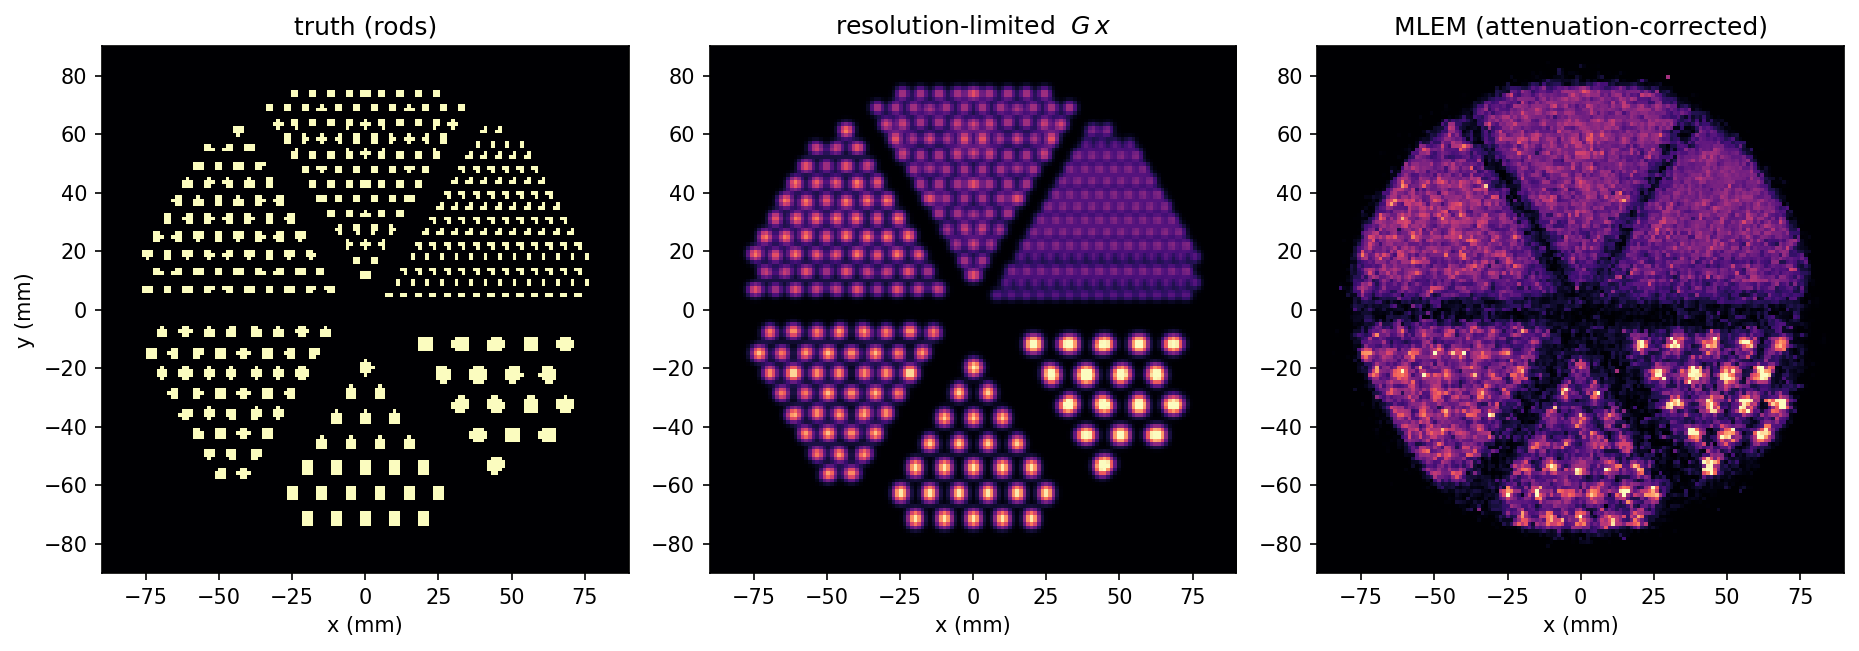
\includegraphics[width=\textwidth]{figures/resolution_result.png}
  \caption{Derenzo phantom, central slice. Left: the sharp truth. Centre: the
    resolution-limited image $\Gop\,\xv$ that the detector can recover. Right:
    the attenuation-corrected MLEM reconstruction, which tracks $\Gop\,\xv$ ---
    the $4$--$6\,\mathrm{mm}$ rods resolve, the $2.5$--$3\,\mathrm{mm}$ rods
    merge at the $3.5\,\mathrm{mm}$ limit.}
  \label{fig:ex-res}
\end{figure}

\section{Running the example}
\label{sec:ex-res:run}

The code is in \code{tutorial/examples/resolution/}: \code{run.jl},
\code{resolution.toml} (all parameters), \code{resolution\_plot.py}. From the
repository root:
\begin{lstlisting}
julia --project=tutorial/examples/resolution -e \
  'using Pkg; Pkg.develop(path="."); Pkg.instantiate()'   # first time
julia -t auto --project=tutorial/examples/resolution \
  tutorial/examples/resolution/run.jl
python3 tutorial/examples/resolution/resolution_plot.py
\end{lstlisting}
Change the rod diameters, the resolution \code{fwhm}, or the voxel size in the
TOML to explore the limit.

\section{What this leaves out}
\label{sec:ex-res:next}

Attenuation and resolution are now both in place. The remaining physical effects
--- \emph{randoms} and \emph{scatter} --- are additive backgrounds that enter
through the \code{contamination} field, and are added in the following examples
without changing the reconstruction code, only the simulated data
(Part~I, The Complete Data Model)~\cite{crysp2026}.

% tbsrc/references.tex — bibliography (self-contained, no bibtex step).
\begin{thebibliography}{9}

\bibitem{joseph1982}
P.~M. Joseph,
\emph{An improved algorithm for reprojecting rays through pixel images},
IEEE Trans.\ Med.\ Imaging \textbf{1}(3):192--196, 1982.

\bibitem{shepp1982}
L.~A. Shepp and Y.~Vardi,
\emph{Maximum likelihood reconstruction for emission tomography},
IEEE Trans.\ Med.\ Imaging \textbf{1}(2):113--122, 1982.

\bibitem{lange1984}
K.~Lange and R.~Carson,
\emph{EM reconstruction algorithms for emission and transmission tomography},
J.\ Comput.\ Assist.\ Tomogr.\ \textbf{8}(2):306--316, 1984.

\bibitem{hudson1994}
H.~M. Hudson and R.~S. Larkin,
\emph{Accelerated image reconstruction using ordered subsets of projection
data},
IEEE Trans.\ Med.\ Imaging \textbf{13}(4):601--609, 1994.

\bibitem{watson2000}
C.~C. Watson,
\emph{New, faster, image-based scatter correction for 3D PET},
IEEE Trans.\ Nucl.\ Sci.\ \textbf{47}(4):1587--1594, 2000.

\bibitem{moses2011}
W.~W. Moses,
\emph{Fundamental limits of spatial resolution in PET},
Nucl.\ Instrum.\ Methods Phys.\ Res.\ A \textbf{648}:S236--S240, 2011.

\bibitem{schramm2024}
G.~Schramm and K.~Thielemans,
\emph{PARALLELPROJ---an open-source framework for fast calculation of
projections in tomography},
Front.\ Nucl.\ Med.\ \textbf{3}:1324562, 2024.

\end{thebibliography}


\end{document}
